\section{Near Neighbor Search}\label{sec:nn}

Fast retrieval of similar patches is crucial for making
construction of a sizeable patch-based database feasible.
This is essentially near-neighbor retrieval in
relatively high dimensions $3 \cdot n^2$ (1875 for patch size $n=25$).
Image retrieval has been addressed in a number of papers,
including more complex feature respresentations ~\cite{perronnin2010large}.
Our poblem is somewhat different from most of previous work
in that the variability
in small patches is much less than in regular-sized images,
semantic information is irrelevant, and vectors are much shorter
than for regular-sized images.
Thus, we focus on tuning a simple Locality-Sensitive Hashing variant for our
particular application.

\subsection{Locality-Sensitive Hashing}

\begin{figure}[ht!]
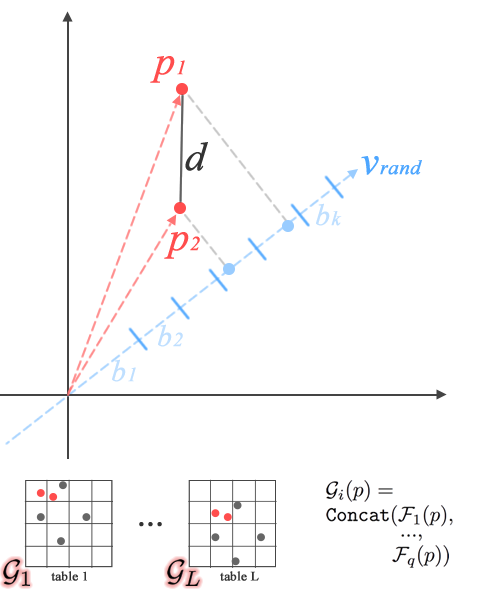
\includegraphics[width=3.0in]{fig_NN/rand_proj_all.png}
\label{fig:lsh}
\caption{Random-projection LSH constructs
$L$ hash tables, each relying on an amplified
hash function $\mathcal{G}$, composed of a concatenation
of simpler hash functions $\mathcal{F}$. Each
$\mathcal{F}$ is evaluated by projecting a point $p$
(a patch color vector in our case) on a randomly chosen
unit vector, and binning it into uniform bins.}
\end{figure}

Locality-Sensitive Hashing (LSH)~\cite{LSH:Andoni}
is a popular approach for approximate near-neighbor search
in high dimensions. The high-level idea behind LSH is
coming up with a set of hashing functions that map
a vector $P_i$ to its bin $b(P_i)$ such that:
\begin{equation*}
\begin{aligned}
P[b(P_i) = b(P_j) | S(P_i, P_j < T)] > P_1\\
P[b(P_i) = b(P_j) | S(P_i, P_j) > cT] < P_2
\end{aligned}
\end{equation*}
The idea is to have high probability of collisions ($> P_1$) for
vectors that are close together, and low probability of collisions
for vectors that are further apart $< P_2$.

In principle hashing-based, it is
attractive for database applications, where entire lookup data structure
cannot be stored in memory.

At a high-level, LSH applies a family of hash functions $F_i$:

Why we don't want many hash tables:






\begin{figure}[ht!]
\subfigure[PCA-based hashing]{%
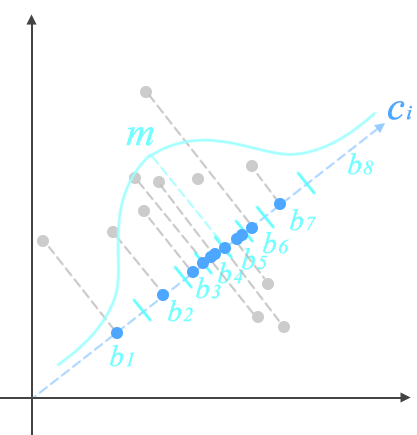
\includegraphics[width=3.0in]{fig_NN/pca_proj.png}
\label{fig:pca-proj}}
\qquad
\subfigure[Dot product distributions]{
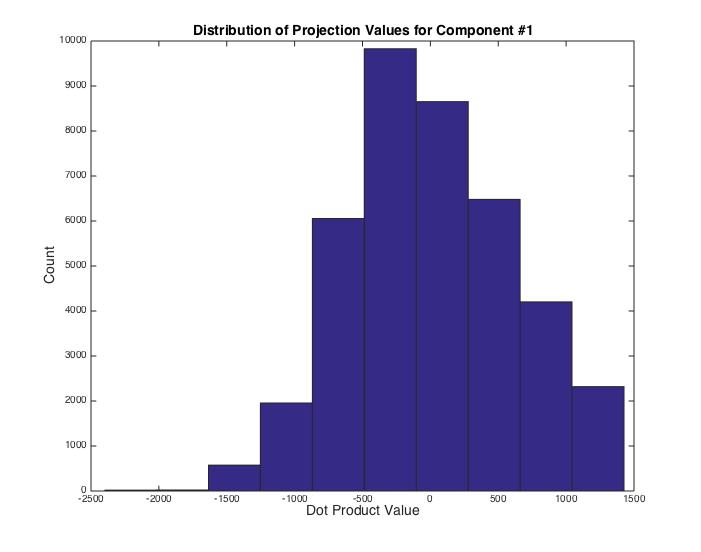
\includegraphics[width=1.0in]{fig_NN/hist_pp1.jpg}
%\vspace{2ex}
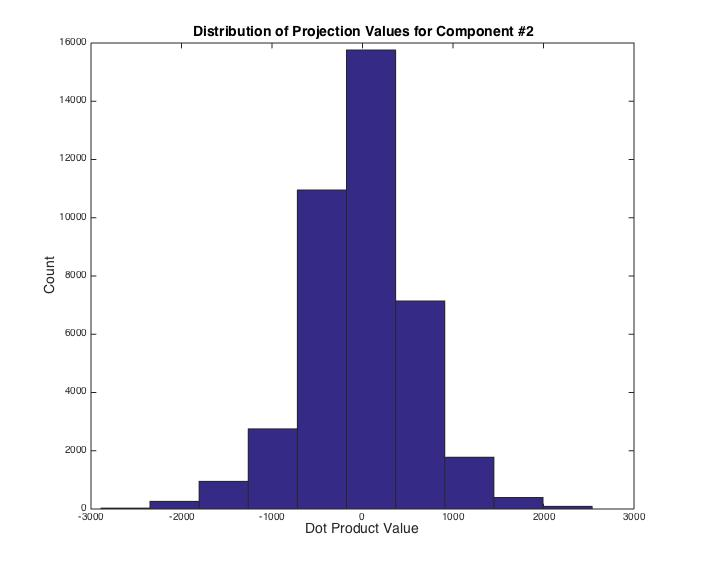
\includegraphics[width=1.0in]{fig_NN/hist_pp2.jpg}
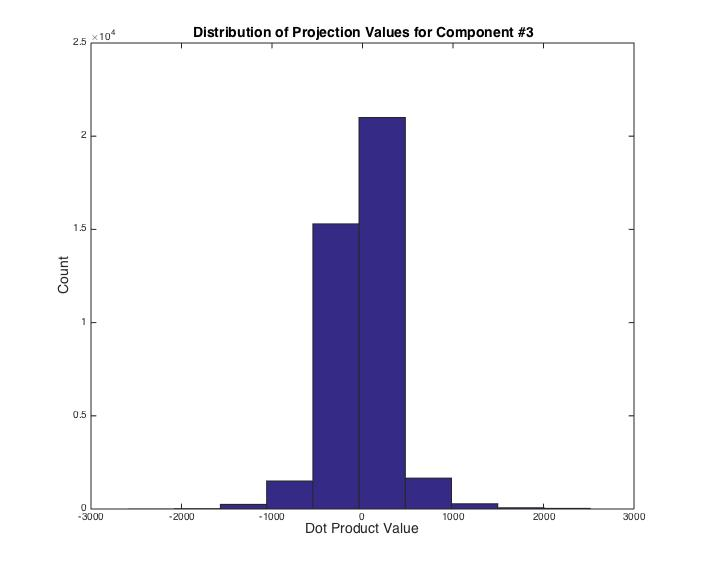
\includegraphics[width=1.0in]{fig_NN/hist_pp3.jpg}
}
\caption{TODO.}

\end{figure}

\subsection{Near-Neighbor Search with LSH}\label{ssec:nn-lsh}

Using a single amplified hash function $\mathcal{G}$, finding
all likely neighbors of a patch simply amounts to computing
its hash value and taking all the patches that fall into the
same hash bin.
Moreformally, we can define the function
in Alg.~\ref{alg:insert2} as follows:
\begin{algorithmic}[1]
\Statex \texttt{\textbf{FindLikelySimilarPatches}}($P_j$):
\State $h \leftarrow \mathcal{G}$ (\texttt{ToVector($P_j$)})
\State $SimPat \leftarrow$ \texttt{select patch from patch\_dict where id in
(select patch\_id from patch\_hashes where hash = h)}
\end{algorithmic}
Of course, the quality of the result depends heavily on the
properties of the hash function, which is something we discuss next.

\subsection{Naive LSH}\label{sec:naive-nn}

\subsection{PCA-based LSH}

\begin{figure}[ht!]
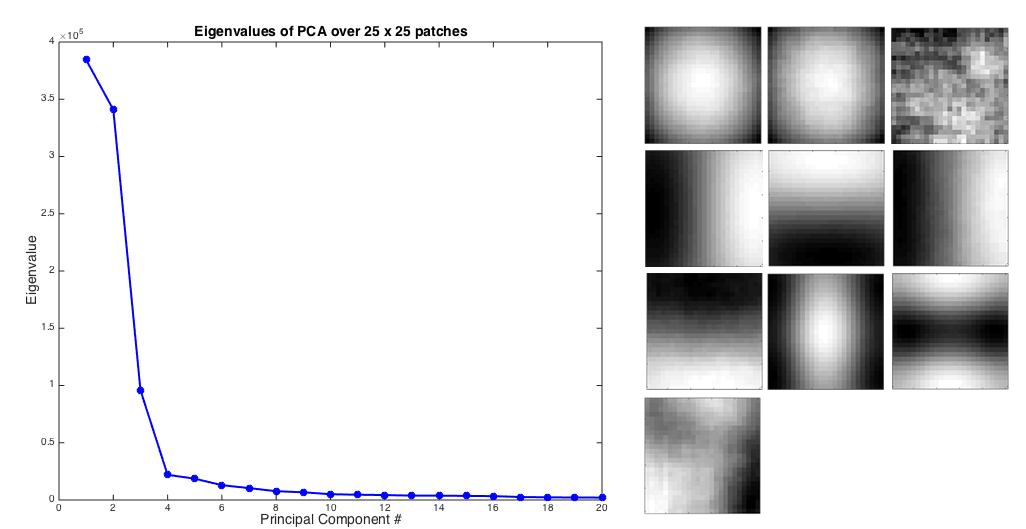
\includegraphics[width=3.0in]{fig_NN/principal_comps.png}
\label{fig:lambdas}
\caption{Eigenvalues of the PCA on 80K patches and visualization
of the L-channel (lightness) of the first 10 components.}
\end{figure}

% PCA-based LHS;\\
% 3 distributions\\
% all components

We ran Principal Component Analysis (PCA) on 80K patch vectors
sampled from 1000 images
sampled uinformly from all the categories in the
SUN database~\cite{SUN}.


\subsection{Color Uniformity}

\begin{figure}[ht!]
\subfigure[Pitfalls of standard deviation]{
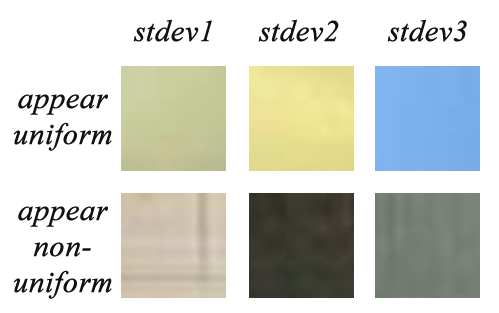
\includegraphics[width=2.7in]{fig_NN/std_uni.png}
\label{fig:color-stdev}}
\subfigure[Uniformity classification with p-norm]{
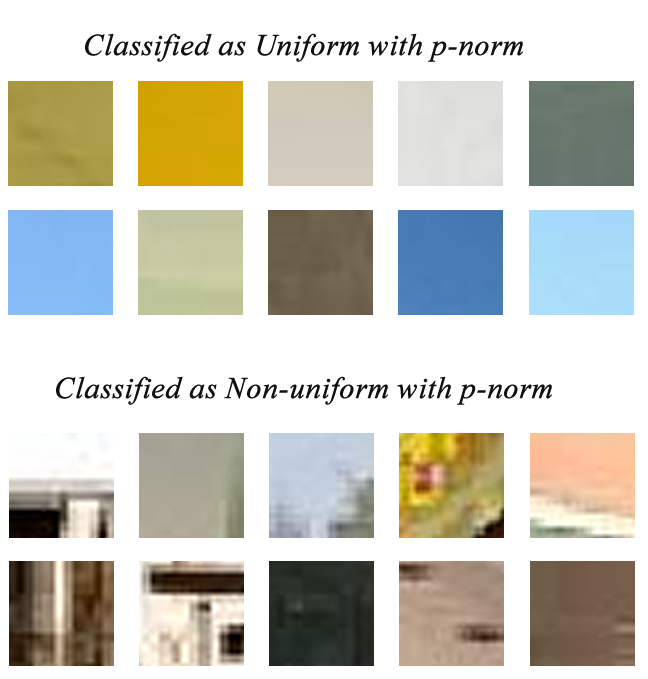
\includegraphics[width=3.5in]{fig_NN/uni_class.png}
\label{fig:color-pnorm}}
\caption{Standard deviation in a) is not very sensitive
to outliers, as patches with nearly identical
values of $stdev1$, $stdev2$ and $stdev3$ may appear
either uniform or non-uniform, as shown in the table.
In b), our classification of patches using
p-norm anecdotally shows more reliable results.}
\end{figure}
